
\documentclass[journal,12pt,twocolumn]{IEEEtran}

\usepackage{setspace}
\usepackage{gensymb}

\singlespacing


\usepackage[cmex10]{amsmath}

\usepackage{amsthm}

\usepackage{mathrsfs}
\usepackage{txfonts}
\usepackage{stfloats}
\usepackage{bm}
\usepackage{cite}
\usepackage{cases}
\usepackage{subfig}

\usepackage{longtable}
\usepackage{multirow}
\DeclareMathOperator{\taninv}{tan\,inverse}
\usepackage{enumitem}
\usepackage{mathtools}
\usepackage{steinmetz}
\usepackage{tikz}
\usepackage{circuitikz}
\usepackage{verbatim}
\usepackage{tfrupee}
\usepackage[breaklinks=true]{hyperref}
\usepackage{graphicx}
\usepackage{tkz-euclide}
\usepackage{float}

\usetikzlibrary{calc,math}
\usepackage{listings}
    \usepackage{color}                                            %%
    \usepackage{array}                                            %%
    \usepackage{longtable}                                        %%
    \usepackage{calc}                                             %%
    \usepackage{multirow}                                         %%
    \usepackage{hhline}                                           %%
    \usepackage{ifthen}                                           %%
    \usepackage{lscape}     
\usepackage{multicol}
\usepackage{chngcntr}

\DeclareMathOperator*{\Res}{Res}

\renewcommand\thesection{\arabic{section}}
\renewcommand\thesubsection{\thesection.\arabic{subsection}}
\renewcommand\thesubsubsection{\thesubsection.\arabic{subsubsection}}

\renewcommand\thesectiondis{\arabic{section}}
\renewcommand\thesubsectiondis{\thesectiondis.\arabic{subsection}}
\renewcommand\thesubsubsectiondis{\thesubsectiondis.\arabic{subsubsection}}


\hyphenation{op-tical net-works semi-conduc-tor}
\def\inputGnumericTable{}                                 %%

\lstset{
%language=C,
frame=single, 
breaklines=true,
columns=fullflexible
}
\begin{document}
\newtheorem{theorem}{Theorem}[section]
\newtheorem{problem}{Problem}
\newtheorem{proposition}{Proposition}[section]
\newtheorem{lemma}{Lemma}[section]
\newtheorem{corollary}[theorem]{Corollary}
\newtheorem{example}{Example}[section]
\newtheorem{definition}[problem]{Definition}

\newcommand{\BEQA}{\begin{eqnarray}}
\newcommand{\EEQA}{\end{eqnarray}}
\newcommand{\define}{\stackrel{\triangle}{=}}
\bibliographystyle{IEEEtran}
\providecommand{\mbf}{\mathbf}
\providecommand{\pr}[1]{\ensuremath{\Pr\left(#1\right)}}
\providecommand{\qfunc}[1]{\ensuremath{Q\left(#1\right)}}
\providecommand{\sbrak}[1]{\ensuremath{{}\left[#1\right]}}
\providecommand{\lsbrak}[1]{\ensuremath{{}\left[#1\right.}}
\providecommand{\rsbrak}[1]{\ensuremath{{}\left.#1\right]}}
\providecommand{\brak}[1]{\ensuremath{\left(#1\right)}}
\providecommand{\lbrak}[1]{\ensuremath{\left(#1\right.}}
\providecommand{\rbrak}[1]{\ensuremath{\left.#1\right)}}
\providecommand{\cbrak}[1]{\ensuremath{\left\{#1\right\}}}
\providecommand{\lcbrak}[1]{\ensuremath{\left\{#1\right.}}
\providecommand{\rcbrak}[1]{\ensuremath{\left.#1\right\}}}
\theoremstyle{remark}
\newtheorem{rem}{Remark}
\newcommand{\sgn}{\mathop{\mathrm{sgn}}}
\providecommand{\abs}[1]{\vert#1\vert}
\providecommand{\res}[1]{\Res\displaylimits_{#1}} 
\providecommand{\norm}[1]{\lVert#1\rVert}
%\providecommand{\norm}[1]{\lVert#1\rVert}
\providecommand{\mtx}[1]{\mathbf{#1}}
\providecommand{\mean}[1]{E[ #1 ]}
\providecommand{\fourier}{\overset{\mathcal{F}}{ \rightleftharpoons}}
%\providecommand{\hilbert}{\overset{\mathcal{H}}{ \rightleftharpoons}}
\providecommand{\system}{\overset{\mathcal{H}}{ \longleftrightarrow}}
	%\newcommand{\solution}[2]{\textbf{Solution:}{#1}}
\newcommand{\solution}{\noindent \textbf{Solution: }}
\newcommand{\cosec}{\,\text{cosec}\,}
\providecommand{\dec}[2]{\ensuremath{\overset{#1}{\underset{#2}{\gtrless}}}}
\newcommand{\myvec}[1]{\ensuremath{\begin{pmatrix}#1\end{pmatrix}}}
\newcommand{\mydet}[1]{\ensuremath{\begin{vmatrix}#1\end{vmatrix}}}
\numberwithin{equation}{subsection}
\makeatletter
\@addtoreset{figure}{problem}
\makeatother
\let\StandardTheFigure\thefigure
\let\vec\mathbf
\renewcommand{\thefigure}{\theproblem}
\def\putbox#1#2#3{\makebox[0in][l]{\makebox[#1][l]{}\raisebox{\baselineskip}[0in][0in]{\raisebox{#2}[0in][0in]{#3}}}}
     \def\rightbox#1{\makebox[0in][r]{#1}}
     \def\centbox#1{\makebox[0in]{#1}}
     \def\topbox#1{\raisebox{-\baselineskip}[0in][0in]{#1}}
     \def\midbox#1{\raisebox{-0.5\baselineskip}[0in][0in]{#1}}
\vspace{3cm}
\title{ASSIGNMENT 5}
\author{RONGALA ARUN SIDDARDHA \\ AI20BTECH110019}
\maketitle
\newpage
\bigskip
\renewcommand{\thefigure}{\theenumi}
\renewcommand{\thetable}{\theenumi}
Download all python codes from 
\begin{lstlisting}
https://github.com/ArunSiddardha/EE3900/blob/main/Assignment_5/code/Assignment_5.py
\end{lstlisting}
%
and latex-tikz codes from 
%
\begin{lstlisting}
https://github.com/ArunSiddardha/EE3900/blob/main/Assignment_5/Assignment_5.tex
\end{lstlisting}
%
\section{Quadratic Forms/Q.2.21}
Find the roots of the quadratic polynomials if they exist \\
a)$$3x^2-5x+2=0$$
b)$$x^2+4x+5=0$$
c)$$2x^2-2\sqrt{2}x+1=0$$
\section{Quadratic Forms/Q.2.21}
Comparing the quadratic equations with standard equation,
\begin{align}
    ax^2+2bxy+cy^2+2dx+2ey+f=0\\
    \therefore c=b=0,e=-\frac{1}{2}, a=3,d=\frac{-5}{2},f=2.\\
    \therefore \vec{V}=\myvec{a & b \\ b & c}=\myvec{3 & 0 \\ 0 & 0}\\ \therefore \vec{u}=\myvec{d \\ e}= \myvec{\frac{-5}{2} \\ \frac{-1}{2}}\\ f=2
\end{align}
 Finding the eigen values corresponding to  $\vec{V}$
\begin{align}
    \mid \vec{V}- \lambda \vec{I} \mid =0\\
    \myvec{ 3- \lambda & 0 \\ 0 & -\lambda}=0\\
    \brak{3 - \lambda}\brak{-\lambda}=0 \\
    \therefore \lambda = 0 ,3 
\end{align}
Calculating the eigen vectors corresponding to the $\lambda$ = 0 ,3 respectively,
\begin{align}
    \vec{V}\vec{x}=\lambda\vec{x}\\
    \myvec{3 & 0 \\ 0 & 0}\vec{x}=0 \implies \vec{p_{1}}=\myvec{0 \\1}\\
    \myvec{0 & 0 \\ 0 & -3}\vec{x} = 3\vec{x} \implies \vec{p_{2}}= \myvec{1 \\ 0} \\
\end{align}
Now by eigen decomposition on $\vec{V}$,
\begin{align}
    \vec{V}= \vec{P}\vec{D}\vec{P}^{\top}\\
    where,\vec{P}= \myvec{\vec{p_{1}}&\vec{p_{2}}}\\
    \vec{P}=\myvec{ 0 & 1 \\ 1 & 0}\\
    \vec{D}= \myvec{\lambda_{1} & 0 \\ 0 & \lambda_{2}}\\
    \vec{D}= \myvec{0 & 0 \\ 0 & 3}
\end{align}
Hence equation becomes,
\begin{align}
    \vec{V}= \myvec{ 0 & 1 \\ 1 & 0}\myvec{0 & 0 \\ 0 & 3}\myvec{ 0 & 1 \\ 1 & 0}\\
    \therefore \vec{V}=\myvec{3 & 0 \\ 0 & 0}
\end{align}
To find the vertex of the parabola ,
\begin{align}
    \myvec{\vec{u}^{\top}+ \eta \vec{p_1}^{\top} \\ \vec{V}}\vec{c} = \myvec{-f \\ \eta \vec{p_1}-\vec{u}}\\
    where, \eta = \vec{u}^{\top}\vec{p_1}= \frac{-1}{2}\\
    \implies
    \vec{c}&=\myvec{-\frac{5}{2}& -1 \\ 3 & 0 \\ 0 & 0}\\ \implies \vec{c}& = \myvec{-2 \\ \frac{5}{2}\\ 0}\\ \implies
    \vec{c}&=\myvec{\frac{5}{6} \\\frac{-1}{12}}
\end{align}
\begin{align}
    \because \vec{p_1}^{\top}\vec{c} &= \myvec{0 & 1}\myvec{\frac{5}{6} \\\frac{-1}{12}}\\
    &= \frac{-1}{12}
\end{align}
and,
\begin{align}
    \vec{p_2}^{\top}\vec{V}\vec{p_2}&= \myvec{1 & 0}\myvec{3 & 0 \\ 0 & 0}\myvec{1 \\ 0}\\
    &= 3\\
    \because (\vec{p_1}^{\top}\vec{c}) (\vec{p_2}^{\top}\vec{V}\vec{p_2})&=\frac{-1}{4}<0 
\end{align}
Hence, The given equation has real roots.\\
\begin{figure}[htp]
    \centering
    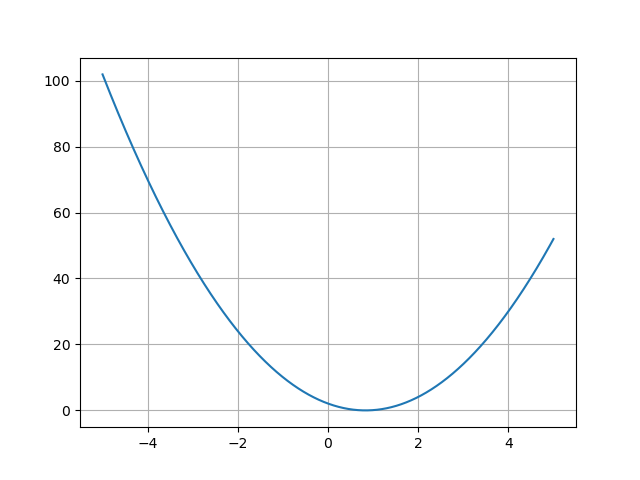
\includegraphics[width=\columnwidth]{Figure_1.png}
    \caption{$3x^2-5x+2$}
\end{figure}
\textbf{ii)}
Comparing the quadratic equations with standard equation,
\begin{align}
    ax^2+&2hxy+by^2+2dx+2ey+f=0\\
    \therefore c&=b,e=\frac{-1}{2}, a=1,d=2,f=5.\\
    \therefore \vec{V}&=\myvec{a & b \\ b & c}=\myvec{1 & 0 \\ 0 & 0}\\ \therefore \vec{u}&=\myvec{d \\ e}= \myvec{2 \\ \frac{-1}{2}}\\ f&=5
\end{align}
Finding the eigen values corresponding to  $\vec{V}$
\begin{align}
    \mid \vec{V}- \lambda \vec{I} \mid &=0\\
    \myvec{ 1- \lambda & 0 \\ 0 & -\lambda}&=0\\
    \brak{1 - \lambda}\brak{-\lambda}&=0 \\
    \therefore \lambda &= 0 ,1 
\end{align}
Calculating the eigen vectors corresponding to the $\lambda$ = 0 ,1 respectively,
\begin{align}
    \vec{V}\vec{x}&=\lambda\vec{x}\\
    \myvec{1 & 0 \\ 0 & 0}\vec{x}&=0 \implies \vec{p_{1}}=\myvec{0 \\1}\\
    \myvec{0 & 0 \\ 0 & -1}\vec{x} &= \vec{x} \implies \vec{p_{2}}= \myvec{1 \\ 0} 
\end{align}
Now by eigen decomposition on $\vec{V}$,
\begin{align}
    \vec{V}&= \vec{P}\vec{D}\vec{P}^{\top}\\
    where,\vec{P}&= \myvec{\vec{p_{1}}&\vec{p_{2}}}\\
    \vec{P}&=\myvec{ 0 & 1 \\ 1 & 0}\\
    \vec{D}&= \myvec{\lambda_{1} & 0 \\ 0 & \lambda_{2}}\\
    \vec{D}&= \myvec{0 & 0 \\ 0 & 1}
\end{align}
Hence equation becomes,
\begin{align}
    \vec{V}&= \myvec{ 0 & 1 \\ 1 & 0}\myvec{0 & 0 \\ 0 & 1}\myvec{ 0 & 1 \\ 1 & 0}\\
    \therefore \vec{V}&=\myvec{1 & 0 \\ 0 & 0}
\end{align}
To find the vertex of the parabola ,
\begin{align}
    \myvec{\vec{u}^{\top}+ \eta \vec{p_1}^{\top} \\ \vec{V}}\vec{c} &= \myvec{-f \\ \eta \vec{p_1}-\vec{u}}\\
    where, \eta &= \vec{u}^{\top}\vec{p_1}\\
    \implies
    \vec{c}&=\myvec{2\\1}
\end{align}
\begin{align}
    \because \vec{p_1}^{\top}\vec{c} &= \myvec{0 & 1}\myvec{2\\1} \\
    &= 1
\end{align}
and,
\begin{align}
    \vec{p_2}^{\top}\vec{V}\vec{p_2}&= \myvec{1 & 0}\myvec{1 & 0 \\ 0 & 0}\myvec{1 \\ 0}\\
    &= 1\\
    \because (\vec{p_1}^{\top}\vec{c}) (\vec{p_2}^{\top}\vec{V}\vec{p_2})=1>0 
\end{align}
Hence, The given equation does not have real roots.\\
\begin{figure}[htp]
    \centering
    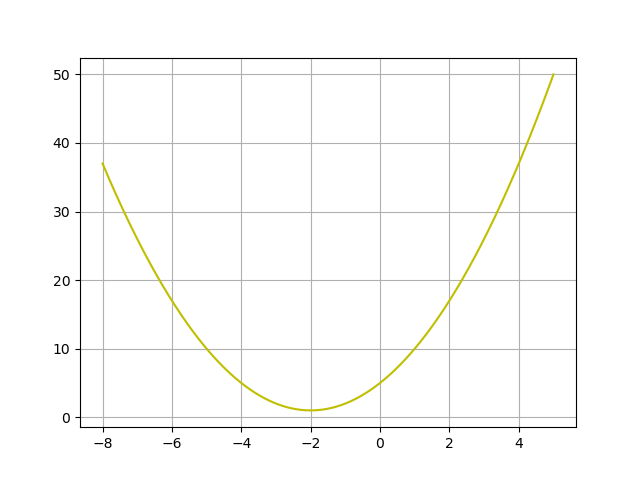
\includegraphics[width=\columnwidth]{Figure_2.png}
    \caption{$x^2+4x+5=0$}
    \label{fig:my_label}
\end{figure}
\textbf{iii)}
Comparing the quadratic equations with standard equation,
\begin{align}
    ax^2+&2hxy+by^2+2dx+2ey+f=0\\
    \therefore c&=b=0,e=\frac{-1}{2}, a=2,d=-\sqrt{2},f=1.\\
    \therefore \vec{V}&=\myvec{2 & b \\ b & c}=\myvec{1 & 0 \\ 0 & 0}\\ \therefore \vec{u}&=\myvec{d \\ e}= \myvec{-\sqrt{2} \\ -\frac{1}{2}}\\ f&=1
\end{align}
Finding the eigen values corresponding to  $\vec{V}$
\begin{align}
    \mid \vec{V}- \lambda \vec{I} \mid &=0\\
    \myvec{ 2- \lambda & 0 \\ 0 & -\lambda}&=0\\
    \brak{2 - \lambda}\brak{-\lambda}&=0 \\
    \therefore \lambda &= 0 ,2
\end{align}
Calculating the eigen vectors corresponding to the $\lambda$ = 0 ,1 respectively,
\begin{align}
    \vec{V}\vec{x}&=\lambda\vec{x}\\
    \myvec{2 & 0 \\ 0 & 0}\vec{x}&=0 \implies \vec{p_{1}}=\myvec{0 \\1}\\
    \myvec{0 & 0 \\ 0 & -2}\vec{x} &= \vec{x} \implies \vec{p_{2}}= \myvec{1 \\ 0} 
\end{align}
Now by eigen decomposition on $\vec{V}$,
\begin{align}
    \vec{V}&= \vec{P}\vec{D}\vec{P}^{\top}\\
    where,\vec{P}&= \myvec{\vec{p_{1}}&\vec{p_{2}}}\\
    \vec{P}&=\myvec{ 0 & 1 \\ 1 & 0}\\
    \vec{D}&= \myvec{\lambda_{1} & 0 \\ 0 & \lambda_{2}}\\
    \vec{D}&= \myvec{0 & 0 \\ 0 & 2}
\end{align}
Hence equation becomes,
\begin{align}
    \vec{V}&= \myvec{ 0 & 1 \\ 1 & 0}\myvec{0 & 0 \\ 0 & 2}\myvec{ 0 & 1 \\ 1 & 0}\\
    \therefore \vec{V}&=\myvec{2 & 0 \\ 0 & 0}
\end{align}
To find the vertex of the parabola ,
\begin{align}
    \myvec{\vec{u}^{\top}+ \eta \vec{p_1}^{\top} \\ \vec{V}}\vec{c} &= \myvec{-f \\ \eta \vec{p_1}-\vec{u}}\\
    where, \eta &= \vec{u}^{\top}\vec{p_1}\\
    \implies
    \vec{c}&=\myvec{\frac{1}{\sqrt{2}}\\0}
\end{align}
\begin{align}
    \because \vec{p_1}^{\top}\vec{c} &= \myvec{0 & 1}\myvec{\frac{1}{\sqrt{2}}\\0} \\
    &= 0
\end{align}
and,
\begin{align}
    \vec{p_2}^{\top}\vec{V}\vec{p_2}&= \myvec{1 & 0}\myvec{1 & 0 \\ 0 & 0}\myvec{1 \\ 0}\\
    &= 1\\
    \because (\vec{p_1}^{\top}\vec{c}) (\vec{p_2}^{\top}\vec{V}\vec{p_2})=0=0 
\end{align}
Hence, The given equation has equal real roots.
\begin{figure}[htp]
    \centering
    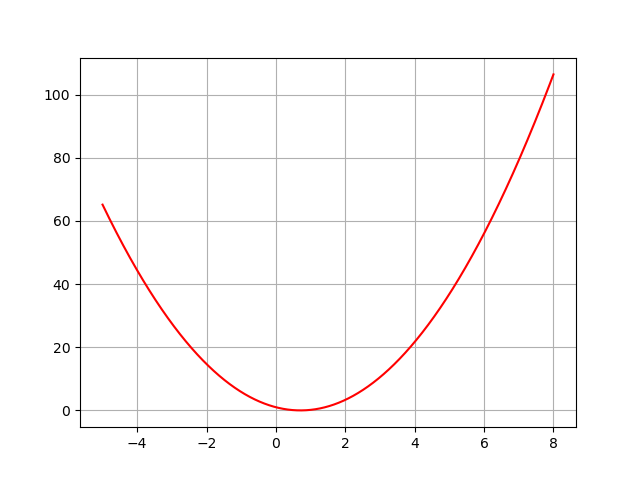
\includegraphics[width=\columnwidth]{Figure_3.png}
    \caption{$2x^2-2\sqrt{2}x+1=0$}
\end{figure}
\end{document}